\section{SIEM}
Heisst: \textbf{Security Information and Event Management}\\

Sicherheitsinformations- und Ereignisverwaltungslösungen sind dafür zuständig, Protokoll- und Ereignisdaten aus verschiedenen Quellen wie Netzwerken, Servern und Anwendungen zu sammeln und in Echtzeit zu aggregieren, zu identifizieren, zu kategorisieren und zu analysieren.
Mit einer SIEM-Lösung sollten Sicherheitsprobleme automatisch erkannt werden und die Möglichkeit bestehen, eine Warnung zu versenden.\\

Ein SIEM macht folgende Dinge:
\begin{itemize}
  \item Ermöglicht die Mustersuche in Protokolldaten nach Indikatoren für einen Cyberangriff (IOC).
  \item Ermöglicht die Korrelation von Ereignisinformationen und identifiziert abnormale Aktivitäten.
  \item Warnt gemäß definierter Warnregeln.
\end{itemize}

\subsubsection{Produkte}
Zum siebten Mal in Folge wurde Splunk von Gartner als Leader im Magic Quadrant 2021 für Security Information and Event Management (SIEM) eingestuft.\\
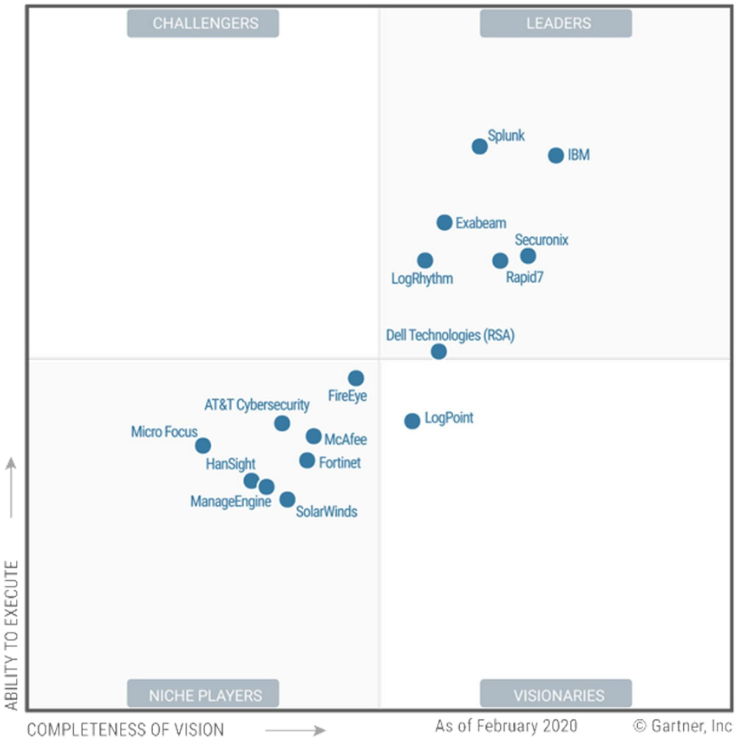
\includegraphics[width=0.8\linewidth]{siem-ranking.png}

\subsubsection{Sigma}
Sigma ist ein generisches und offenes Signaturformat, mit dem Sie relevante Protokollereignisse auf einfache Weise beschreiben können. Das Regelformat ist sehr flexibel, leicht zu schreiben und auf jede Art von Protokolldateien anwendbar. Das Hauptziel dieses Projekts ist es, eine strukturierte Form bereitzustellen, in der Forscher oder Analysten ihre einmal entwickelten Erkennungsmethoden beschreiben und mit anderen teilen können.\\
\textit{Sigma} ist für Logs das, was Snort für den Netzwerkverkehr und YARA für Dateien ist.\\
\textbf{Use-Cases}
\begin{itemize}
    \item Describe your detection method in Sigma to make it shareable
    \item YAML based
    \item Write your SIEM searches in Sigma to avoid a vendor lock-in
    \item Share the signature in the appendix of your analysis along with IOCs and YARA rules
    \item Share the signature in threat intel communities - e.g. via MISP
    \item Provide Sigma signatures for malicious behaviour in your own application
\end{itemize}


\subsection{Wazuh}
Wazuh ist eine Open-Source-Sicherheitsplattform, die sich auf die Überwachung der Infrastruktur, die Erkennung von Sicherheitsrisiken und die Reaktion auf Vorfälle im Sinne eines SIEM und EDR (Endpoint Detection \& Response) konzentriert.\\

Der sogenannte Wazuh-Agent wird auf den zu überwachenden Maschinen installiert und kommuniziert mit dem Wazuh-Manager, der auf einem Server installiert ist.
Der Wazuh-Manager empfängt und analysiert Daten von den Agenten unter Verwendung von Decodern und Regeln, die zur Auslösung von Sicherheitswarnungen erstellt wurden.
Der Manager dient auch dazu, Konfigurationsdateien an die Agenten zu verteilen, ihren Status zu überwachen und Kontrollmeldungen zu senden, um automatische Aktionen auf Agentenebene auszulösen.
Damit die Daten übersichtlich dargestellt werden, werden sie weiter an Komponenten von Elastic Stack gesendet und mit Kibana in einem Dashboard angezeigt.

\subsubsection{Architektur}
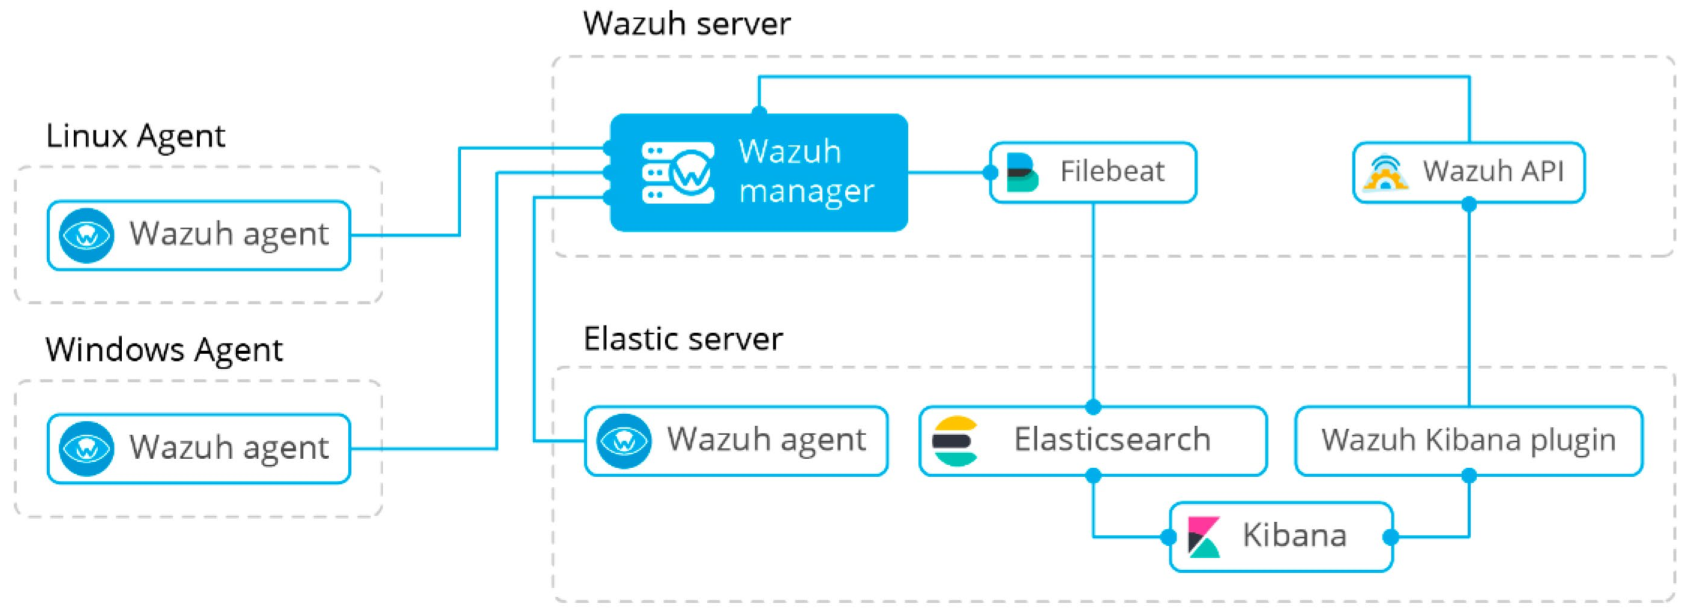
\includegraphics[width=\linewidth]{wazuh-architecture.png}\\
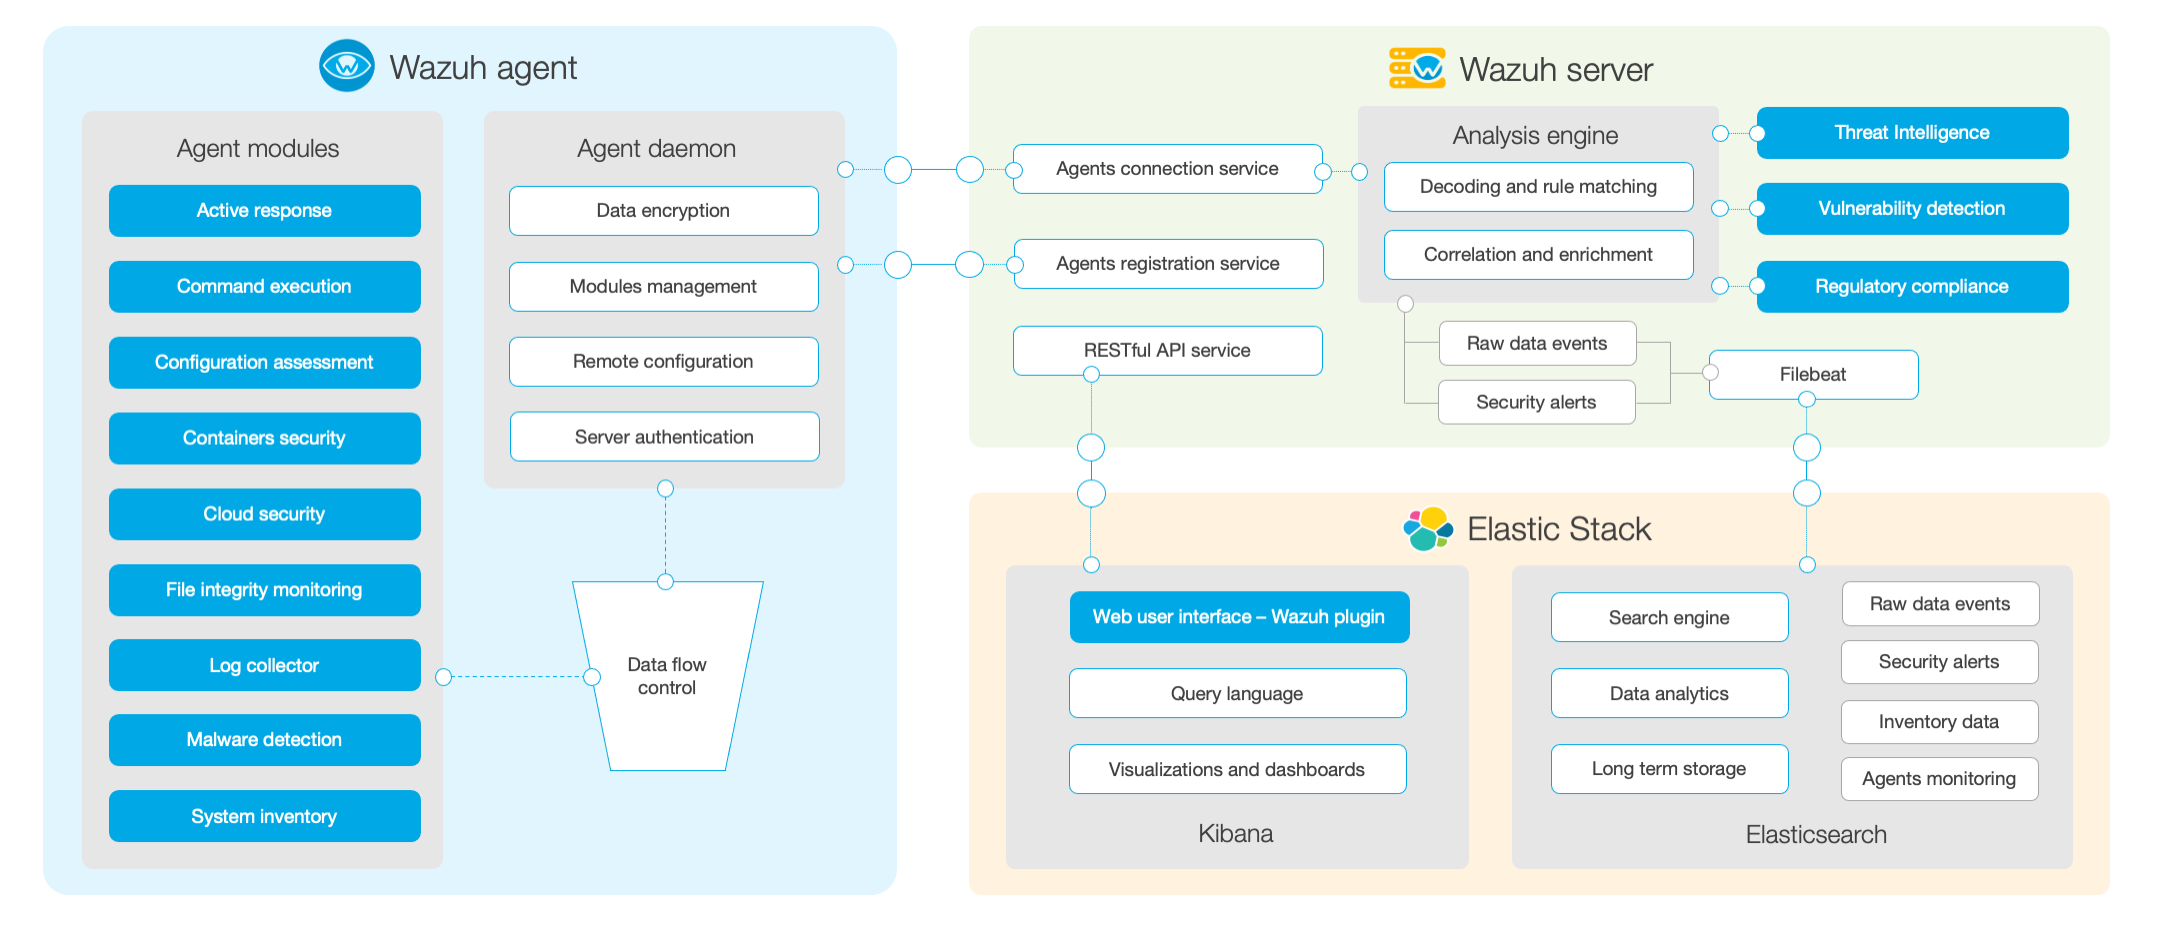
\includegraphics[width=\linewidth]{wazuh-stack.png}

\subsubsection{Wazuh Agent}
Der Wazuh-Agent läuft auf Linux, Windows, macOS, Solaris, AIX und anderen Betriebssystemen.
Er kann auf Laptops, Desktops, Servern, Cloud-Instanzen, Containern oder virtuellen Maschinen eingesetzt werden.
Es bietet Funktionen zur Prävention, Erkennung und Reaktion auf Bedrohungen.
Außerdem sammelt es verschiedene Arten von System- und Anwendungsdaten, die es über einen verschlüsselten und authentifizierten Kanal an den Wazuh-Server weiterleitet.\\

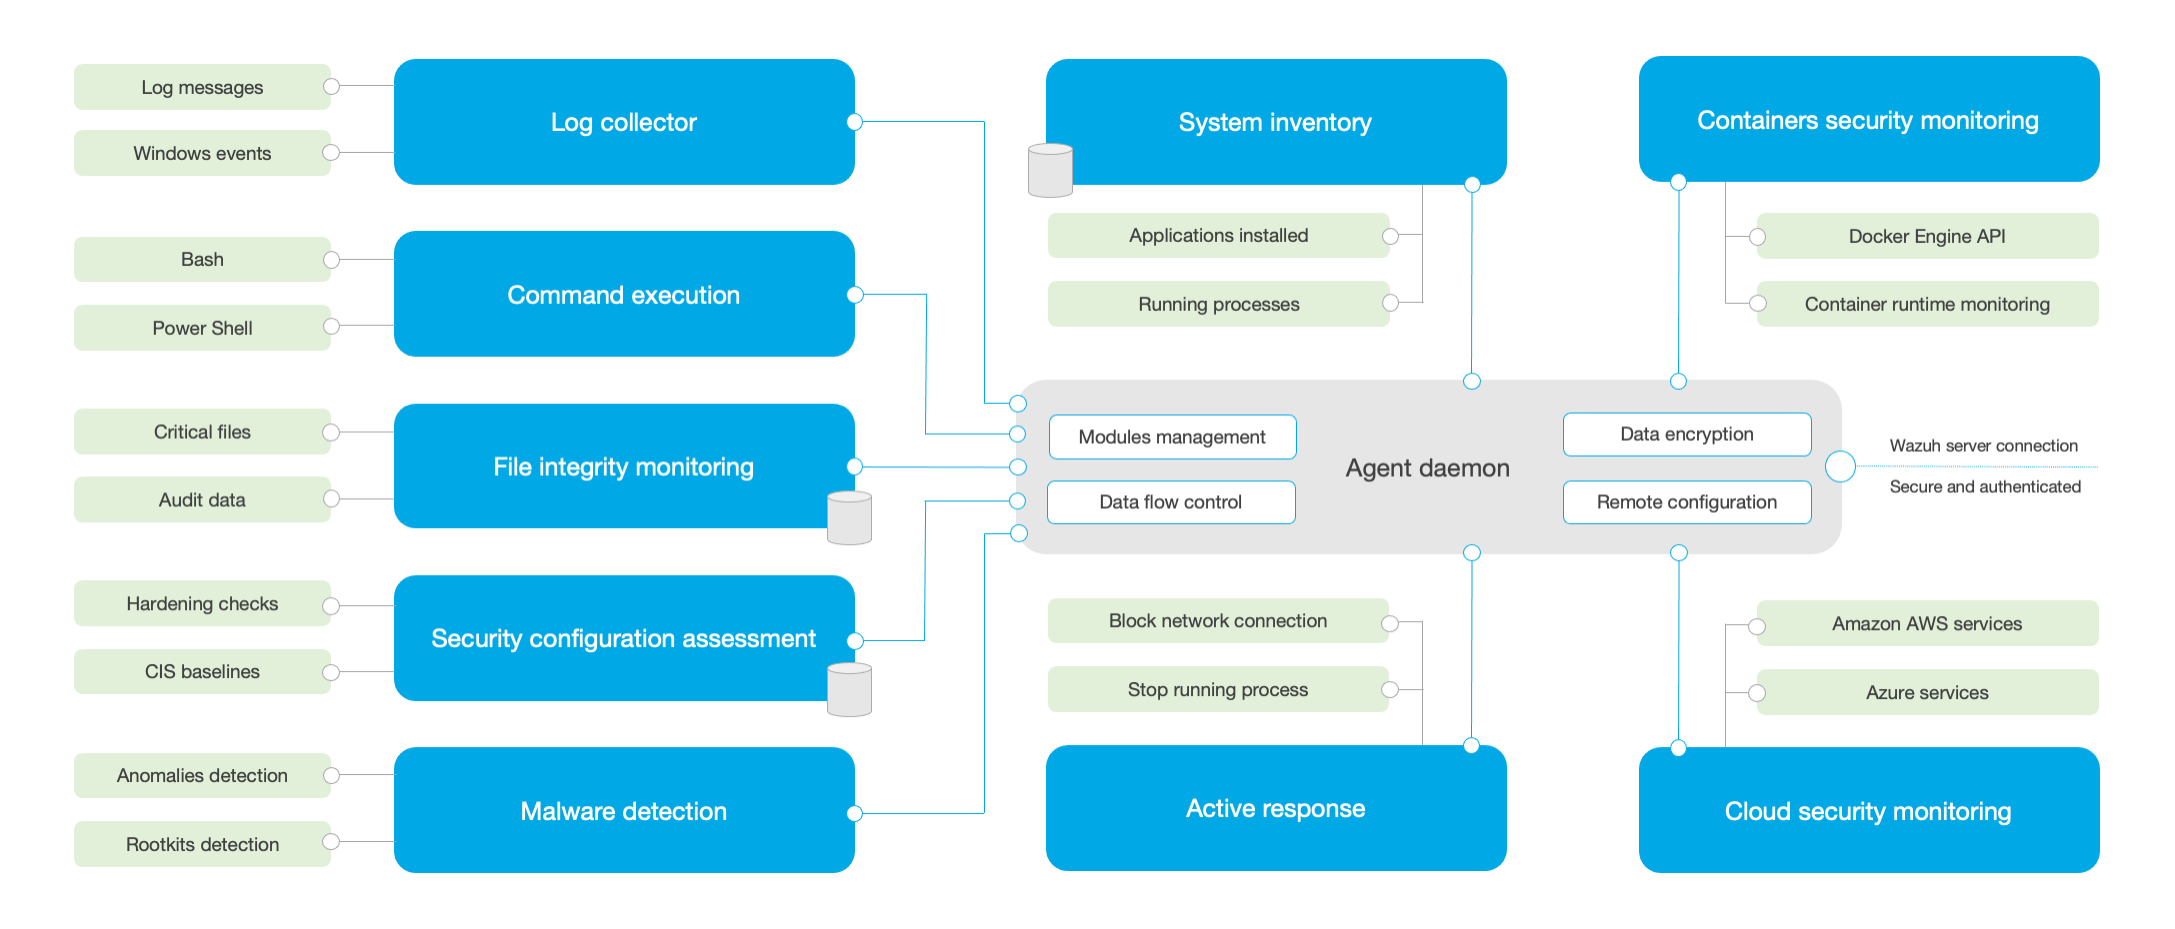
\includegraphics[width=\linewidth]{wazuh-agent-architecture.png}

\paragraph{Agent Module}
\subparagraph{Log Collector}
Diese Komponente kann flache Log-Dateien und Windows-Ereignisse lesen und dabei Betriebssystem- und Anwendungsprotokollmeldungen sammeln. 
Sie unterstützt XPath-Filter für Windows-Ereignisse und erkennt mehrzeilige Formate (z. B. Linux-Audit-Logs). 
Sie kann auch JSON-Ereignisse mit zusätzlichen Metadaten anreichern.

\subparagraph{Command Execution}
Agenten können in regelmäßigen Abständen autorisierte Befehle ausführen, ihre Ausgaben sammeln und sie zur weiteren Analyse an den Wazuh-Server zurückmelden.
Dieses Modul kann für verschiedene Zwecke eingesetzt werden (z. B. Überwachung des verbleibenden Festplattenplatzes, Abrufen einer Liste der zuletzt angemeldeten Benutzer usw.).

\subparagraph{File integrity monitoring (FIM)}
Dieses Modul überwacht das Dateisystem und meldet, wenn Dateien erstellt, gelöscht oder geändert werden. 
Es verfolgt die Dateiattribute, Berechtigungen, Eigentümer und Inhalte. 
Wenn ein Ereignis eintritt, werden die Angaben "wer", "was" und "wann" in Echtzeit erfasst. 
Darüber hinaus erstellt und verwaltet dieses Modul eine Datenbank mit dem Status der überwachten Dateien, so dass Abfragen per Fernzugriff möglich sind.

\subparagraph{Security configuration assessment (SCA)}
Diese Komponente bietet eine kontinuierliche Konfigurationsbewertung, die auf der Grundlage der Benchmarks des Center of Internet Security (CIS) sofort einsatzbereit ist. Benutzer können auch ihre eigenen SCA-Prüfungen erstellen, um ihre Sicherheitsrichtlinien zu überwachen und durchzusetzen.

\subparagraph{System inventory}
Dieses Agentenmodul führt in regelmäßigen Abständen Scans durch und sammelt dabei Bestandsdaten wie Betriebssystemversion, Netzwerkschnittstellen, laufende Prozesse, installierte Anwendungen und eine Liste offener Ports. 
Die Scan-Ergebnisse werden in lokalen SQLite-Datenbanken gespeichert, die per Fernzugriff abgefragt werden können.

\subparagraph{Malware detection}
Mithilfe eines nicht signaturbasierten Ansatzes ist diese Komponente in der Lage, Anomalien und das mögliche Vorhandensein von Rootkits zu erkennen. Sie überwacht Systemaufrufe und sucht nach versteckten Prozessen, versteckten Dateien und versteckten Ports.

\subparagraph{Active response}
Dieses Modul führt automatische Aktionen aus, wenn Bedrohungen erkannt werden. Unter anderem kann es eine Netzwerkverbindung blockieren, einen laufenden Prozess stoppen oder eine bösartige Datei löschen. 
Bei Bedarf können auch benutzerdefinierte Reaktionen erstellt werden (z. B. Ausführen eines Binärprogramms in einer Sandbox, Erfassen des Netzwerkverbindungsverkehrs, Scannen einer Datei mit einem Antivirusprogramm usw.).

\subparagraph{Containers security monitoring}
Dieses Agentenmodul ist in die Docker-Engine-API integriert, um Änderungen in einer containerisierten Umgebung zu überwachen. 
Es erkennt zum Beispiel Änderungen an Container-Images, Netzwerkkonfigurationen oder Datenvolumina. 
Außerdem alarmiert es bei Containern, die im privilegierten Modus laufen, und bei Benutzern, die Befehle in einem laufenden Container ausführen.

\subparagraph{Cloud security monitoring}
Diese Komponente überwacht Cloud-Anbieter wie Amazon AWS, Microsoft Azure oder Google GCP.
Sie kommuniziert nativ mit deren APIs.
Sie ist in der Lage, Änderungen an der Cloud-Infrastruktur zu erkennen (z. B. Erstellung eines neuen Benutzers, Änderung einer Sicherheitsgruppe, Stoppen einer Cloud-Instanz usw.) und Protokolldaten von Cloud-Diensten zu sammeln (z. B. AWS Cloudtrail, AWS Macie, AWS GuardDuty, Azure Active Directory usw.).

\subsubsection{Wazuh Server}
Die Wazuh-Serverkomponente ist für die Analyse der von den Agenten empfangenen Daten zuständig und löst Warnungen aus, wenn Bedrohungen oder Anomalien entdeckt werden.
Sie dient auch dazu, die Konfiguration der Agenten aus der Ferne zu verwalten und ihren Status zu überwachen.\\

Der Wazuh-Server nutzt Quellen für Bedrohungsdaten, um seine Erkennungsfähigkeiten zu verbessern.
Darüber hinaus nutzt er die Compliance-Anforderungen (z.B. PCI DSS, HIPAA, NIST 800-53\dots) und das Mitre ATT\&CK-Framework, um die Alarmdaten anzureichern und ihnen einen nützlichen Kontext zu verleihen.\\

Zusätzlich kann der Wazuh-Server mit externer Software wie Ticketing-Systemen (z.B. Service Now, Jira, PagerDuty) und Instant-Messaging-Plattformen (z.B. Slack) integriert werden. 
Dies ist praktisch, um Sicherheitsabläufe zu rationalisieren.\\

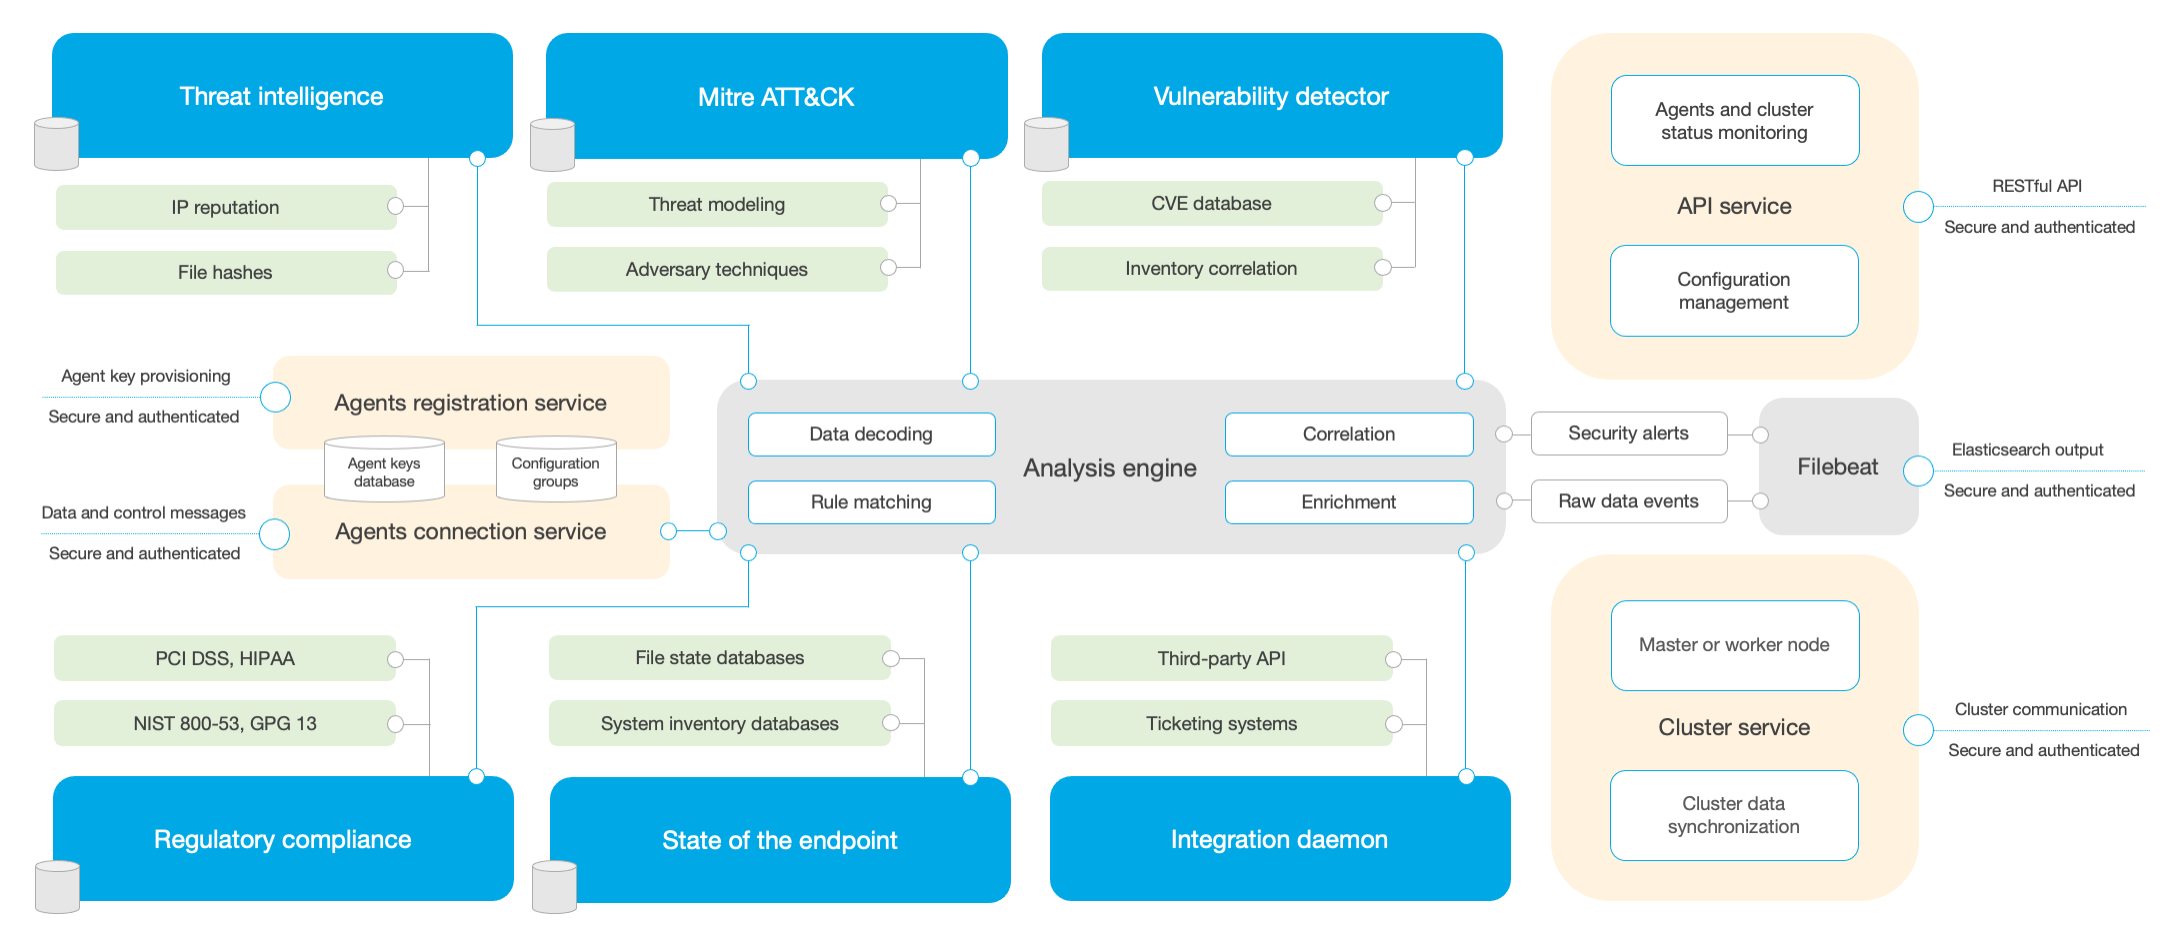
\includegraphics[width=\linewidth]{wazuh-server-architecture.png}

\section{EDR}
Heisst: \textbf{Endpoint detection and response}\\

EDR, auch bekannt als Endpoint Threat Detection and Response (ETDR), ist eine integrierte Endpunkt-Sicherheitslösung, die eine kontinuierliche Überwachung und Erfassung von Endpunktdaten in Echtzeit mit regelbasierten automatischen Reaktions- und Analysefunktionen kombiniert.

\subsection{Produkte}
Microsoft war im 2021 Leader in der Endpoint Protection.\\
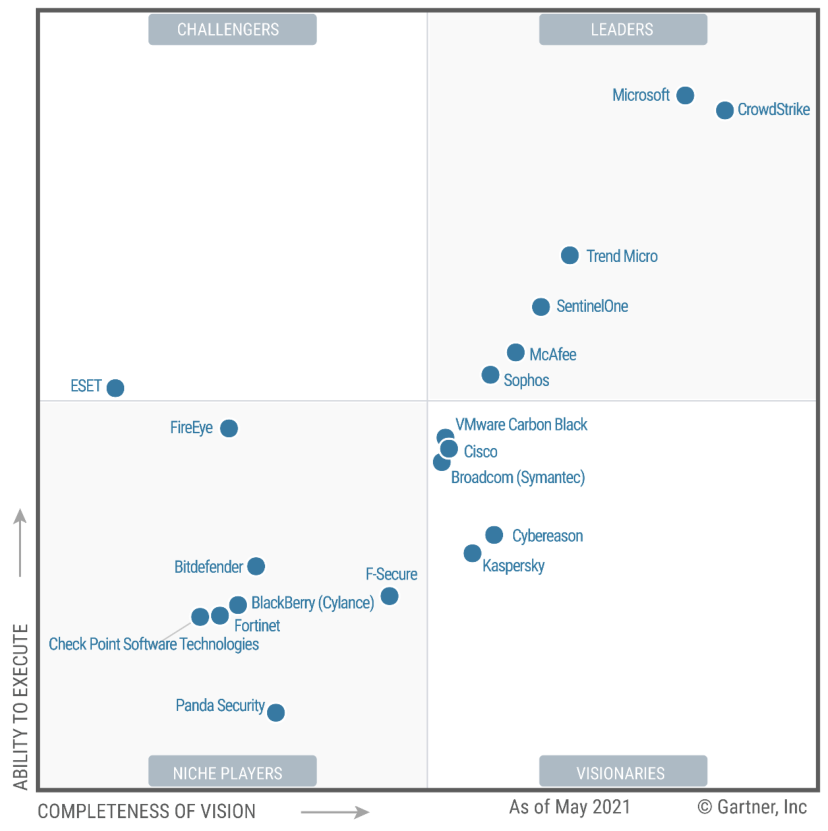
\includegraphics[width=\linewidth]{edr-products.png}